\documentclass[twoside]{book}

% Packages required by doxygen
\usepackage{fixltx2e}
\usepackage{calc}
\usepackage{doxygen}
\usepackage[export]{adjustbox} % also loads graphicx
\usepackage{graphicx}
\usepackage[utf8]{inputenc}
\usepackage{makeidx}
\usepackage{multicol}
\usepackage{multirow}
\PassOptionsToPackage{warn}{textcomp}
\usepackage{textcomp}
\usepackage[nointegrals]{wasysym}
\usepackage[table]{xcolor}

% Font selection
\usepackage[T1]{fontenc}
\usepackage[scaled=.90]{helvet}
\usepackage{courier}
\usepackage{amssymb}
\usepackage{sectsty}
\renewcommand{\familydefault}{\sfdefault}
\allsectionsfont{%
  \fontseries{bc}\selectfont%
  \color{darkgray}%
}
\renewcommand{\DoxyLabelFont}{%
  \fontseries{bc}\selectfont%
  \color{darkgray}%
}
\newcommand{\+}{\discretionary{\mbox{\scriptsize$\hookleftarrow$}}{}{}}

% Page & text layout
\usepackage{geometry}
\geometry{%
  a4paper,%
  top=2.5cm,%
  bottom=2.5cm,%
  left=2.5cm,%
  right=2.5cm%
}
\tolerance=750
\hfuzz=15pt
\hbadness=750
\setlength{\emergencystretch}{15pt}
\setlength{\parindent}{0cm}
\setlength{\parskip}{3ex plus 2ex minus 2ex}
\makeatletter
\renewcommand{\paragraph}{%
  \@startsection{paragraph}{4}{0ex}{-1.0ex}{1.0ex}{%
    \normalfont\normalsize\bfseries\SS@parafont%
  }%
}
\renewcommand{\subparagraph}{%
  \@startsection{subparagraph}{5}{0ex}{-1.0ex}{1.0ex}{%
    \normalfont\normalsize\bfseries\SS@subparafont%
  }%
}
\makeatother

% Headers & footers
\usepackage{fancyhdr}
\pagestyle{fancyplain}
\fancyhead[LE]{\fancyplain{}{\bfseries\thepage}}
\fancyhead[CE]{\fancyplain{}{}}
\fancyhead[RE]{\fancyplain{}{\bfseries\leftmark}}
\fancyhead[LO]{\fancyplain{}{\bfseries\rightmark}}
\fancyhead[CO]{\fancyplain{}{}}
\fancyhead[RO]{\fancyplain{}{\bfseries\thepage}}
\fancyfoot[LE]{\fancyplain{}{}}
\fancyfoot[CE]{\fancyplain{}{}}
\fancyfoot[RE]{\fancyplain{}{\bfseries\scriptsize Generated by Doxygen }}
\fancyfoot[LO]{\fancyplain{}{\bfseries\scriptsize Generated by Doxygen }}
\fancyfoot[CO]{\fancyplain{}{}}
\fancyfoot[RO]{\fancyplain{}{}}
\renewcommand{\footrulewidth}{0.4pt}
\renewcommand{\chaptermark}[1]{%
  \markboth{#1}{}%
}
\renewcommand{\sectionmark}[1]{%
  \markright{\thesection\ #1}%
}

% Indices & bibliography
\usepackage{natbib}
\usepackage[titles]{tocloft}
\setcounter{tocdepth}{3}
\setcounter{secnumdepth}{5}
\makeindex

% Hyperlinks (required, but should be loaded last)
\usepackage{ifpdf}
\ifpdf
  \usepackage[pdftex,pagebackref=true]{hyperref}
\else
  \usepackage[ps2pdf,pagebackref=true]{hyperref}
\fi
\hypersetup{%
  colorlinks=true,%
  linkcolor=blue,%
  citecolor=blue,%
  unicode%
}

% Custom commands
\newcommand{\clearemptydoublepage}{%
  \newpage{\pagestyle{empty}\cleardoublepage}%
}

\usepackage{caption}
\captionsetup{labelsep=space,justification=centering,font={bf},singlelinecheck=off,skip=4pt,position=top}

%===== C O N T E N T S =====

\begin{document}

% Titlepage & ToC
\hypersetup{pageanchor=false,
             bookmarksnumbered=true,
             pdfencoding=unicode
            }
\pagenumbering{alph}
\begin{titlepage}
\vspace*{7cm}
\begin{center}%
{\Large P\+ID Controller Library }\\
\vspace*{1cm}
{\large Generated by Doxygen 1.8.13}\\
\end{center}
\end{titlepage}
\clearemptydoublepage
\pagenumbering{roman}
\tableofcontents
\clearemptydoublepage
\pagenumbering{arabic}
\hypersetup{pageanchor=true}

%--- Begin generated contents ---
\chapter{Hierarchical Index}
\section{Class Hierarchy}
This inheritance list is sorted roughly, but not completely, alphabetically\+:\begin{DoxyCompactList}
\item \contentsline{section}{P\+I\+D\+Controller\+Interface}{\pageref{classPIDControllerInterface}}{}
\begin{DoxyCompactList}
\item \contentsline{section}{Abstract\+P\+I\+D\+Controller}{\pageref{classAbstractPIDController}}{}
\begin{DoxyCompactList}
\item \contentsline{section}{P\+I\+D\+Controller}{\pageref{classPIDController}}{}
\end{DoxyCompactList}
\end{DoxyCompactList}
\end{DoxyCompactList}

\chapter{Class Index}
\section{Class List}
Here are the classes, structs, unions and interfaces with brief descriptions\+:\begin{DoxyCompactList}
\item\contentsline{section}{\hyperlink{classAbstractPIDController}{Abstract\+P\+I\+D\+Controller} \\*\hyperlink{classPIDController}{P\+I\+D\+Controller} abstract class. This contains all the getters and setters required for the member data }{\pageref{classAbstractPIDController}}{}
\item\contentsline{section}{\hyperlink{classPIDController}{P\+I\+D\+Controller} \\*Concrete implementation of the \hyperlink{classPIDController}{P\+I\+D\+Controller} abstract class and interface }{\pageref{classPIDController}}{}
\item\contentsline{section}{\hyperlink{classPIDControllerInterface}{P\+I\+D\+Controller\+Interface} \\*\hyperlink{classPIDController}{P\+I\+D\+Controller} interface will have the \hyperlink{classPIDControllerInterface_a6b5340968cb9d235cf3b52bd61c973e1}{compute()} method. This can be implemented by any concrete class }{\pageref{classPIDControllerInterface}}{}
\end{DoxyCompactList}

\chapter{Class Documentation}
\hypertarget{classAbstractPIDController}{}\section{Abstract\+P\+I\+D\+Controller Class Reference}
\label{classAbstractPIDController}\index{Abstract\+P\+I\+D\+Controller@{Abstract\+P\+I\+D\+Controller}}


\hyperlink{classPIDController}{P\+I\+D\+Controller} abstract class. This contains all the getters and setters required for the member data.  




{\ttfamily \#include $<$pid.\+hpp$>$}



Inheritance diagram for Abstract\+P\+I\+D\+Controller\+:\nopagebreak
\begin{figure}[H]
\begin{center}
\leavevmode
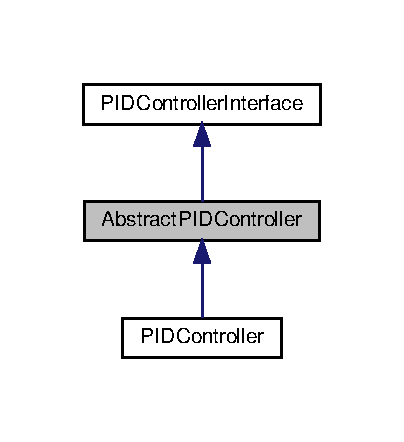
\includegraphics[width=194pt]{classAbstractPIDController__inherit__graph}
\end{center}
\end{figure}


Collaboration diagram for Abstract\+P\+I\+D\+Controller\+:\nopagebreak
\begin{figure}[H]
\begin{center}
\leavevmode
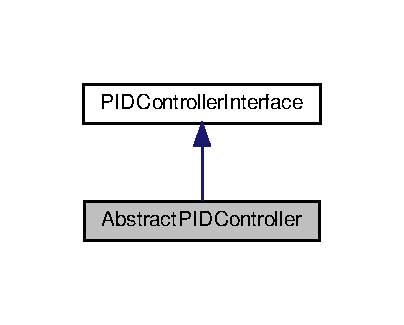
\includegraphics[width=194pt]{classAbstractPIDController__coll__graph}
\end{center}
\end{figure}
\subsection*{Public Member Functions}
\begin{DoxyCompactItemize}
\item 
\mbox{\Hypertarget{classAbstractPIDController_a9eeed269150ef3cf0300a6f2c69e8db5}\label{classAbstractPIDController_a9eeed269150ef3cf0300a6f2c69e8db5}} 
virtual double {\bfseries get\+\_\+dt} () const =0
\item 
\mbox{\Hypertarget{classAbstractPIDController_a9740891451c542659984f36be2f7bf7f}\label{classAbstractPIDController_a9740891451c542659984f36be2f7bf7f}} 
virtual void {\bfseries set\+\_\+dt} (double dt)=0
\item 
\mbox{\Hypertarget{classAbstractPIDController_aa218e356f7c573b7e647d016e424bc8a}\label{classAbstractPIDController_aa218e356f7c573b7e647d016e424bc8a}} 
virtual double {\bfseries get\+\_\+kD} () const =0
\item 
\mbox{\Hypertarget{classAbstractPIDController_acfa3b12144a8d2d890846bcb859def28}\label{classAbstractPIDController_acfa3b12144a8d2d890846bcb859def28}} 
virtual void {\bfseries set\+\_\+kD} (double kD)=0
\item 
\mbox{\Hypertarget{classAbstractPIDController_a86660969fd600fd4f8c338a0fb85e1fc}\label{classAbstractPIDController_a86660969fd600fd4f8c338a0fb85e1fc}} 
virtual double {\bfseries get\+\_\+kI} () const =0
\item 
\mbox{\Hypertarget{classAbstractPIDController_ae1c75f5a3f2c6aa6c2ecdd32e2940552}\label{classAbstractPIDController_ae1c75f5a3f2c6aa6c2ecdd32e2940552}} 
virtual void {\bfseries set\+\_\+kI} (double kI)=0
\item 
\mbox{\Hypertarget{classAbstractPIDController_a4cf58b1bfba161c6c196f42d5e19e805}\label{classAbstractPIDController_a4cf58b1bfba161c6c196f42d5e19e805}} 
virtual double {\bfseries get\+\_\+kP} () const =0
\item 
\mbox{\Hypertarget{classAbstractPIDController_a2e9c6d5a86ce2bb091a7fc35060cb07a}\label{classAbstractPIDController_a2e9c6d5a86ce2bb091a7fc35060cb07a}} 
virtual void {\bfseries set\+\_\+kP} (double kP)=0
\item 
\mbox{\Hypertarget{classAbstractPIDController_aac9cb0e2295e13b73ec17333a840506e}\label{classAbstractPIDController_aac9cb0e2295e13b73ec17333a840506e}} 
virtual double {\bfseries get\+\_\+max\+\_\+value} () const =0
\item 
\mbox{\Hypertarget{classAbstractPIDController_a15bcde3951e0f994adebf926a39a9354}\label{classAbstractPIDController_a15bcde3951e0f994adebf926a39a9354}} 
virtual void {\bfseries set\+\_\+max\+\_\+value} (double max\+Value)=0
\item 
\mbox{\Hypertarget{classAbstractPIDController_a69d79599ae7dcff08fdfedfbd6a15419}\label{classAbstractPIDController_a69d79599ae7dcff08fdfedfbd6a15419}} 
virtual double {\bfseries get\+\_\+min\+\_\+value} () const =0
\item 
\mbox{\Hypertarget{classAbstractPIDController_ad5aaaa7291b6d962a2a472c4b94f6fb2}\label{classAbstractPIDController_ad5aaaa7291b6d962a2a472c4b94f6fb2}} 
virtual void {\bfseries set\+\_\+min\+\_\+value} (double min\+Value)=0
\item 
\mbox{\Hypertarget{classAbstractPIDController_aadecb6cc853ad0b290d178a96ac87aa5}\label{classAbstractPIDController_aadecb6cc853ad0b290d178a96ac87aa5}} 
virtual double {\bfseries get\+\_\+prev\+\_\+error} () const =0
\item 
\mbox{\Hypertarget{classAbstractPIDController_a59157c39c2d62bfb426f7ff3cbcfcb25}\label{classAbstractPIDController_a59157c39c2d62bfb426f7ff3cbcfcb25}} 
virtual double {\bfseries get\+\_\+integral\+\_\+sum} () const =0
\end{DoxyCompactItemize}


\subsection{Detailed Description}
\hyperlink{classPIDController}{P\+I\+D\+Controller} abstract class. This contains all the getters and setters required for the member data. 

The documentation for this class was generated from the following file\+:\begin{DoxyCompactItemize}
\item 
include/pid.\+hpp\end{DoxyCompactItemize}

\hypertarget{classPIDController}{}\section{P\+I\+D\+Controller Class Reference}
\label{classPIDController}\index{P\+I\+D\+Controller@{P\+I\+D\+Controller}}


Concrete implementation of the \hyperlink{classPIDController}{P\+I\+D\+Controller} abstract class and interface.  




{\ttfamily \#include $<$pid.\+hpp$>$}



Inheritance diagram for P\+I\+D\+Controller\+:\nopagebreak
\begin{figure}[H]
\begin{center}
\leavevmode
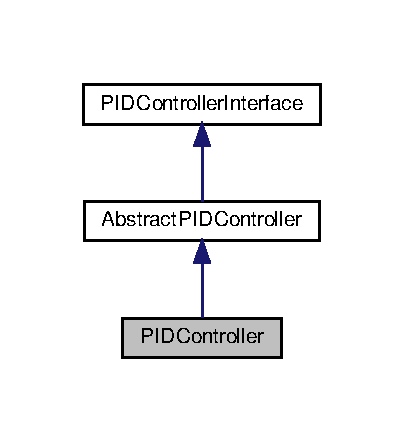
\includegraphics[width=194pt]{classPIDController__inherit__graph}
\end{center}
\end{figure}


Collaboration diagram for P\+I\+D\+Controller\+:\nopagebreak
\begin{figure}[H]
\begin{center}
\leavevmode
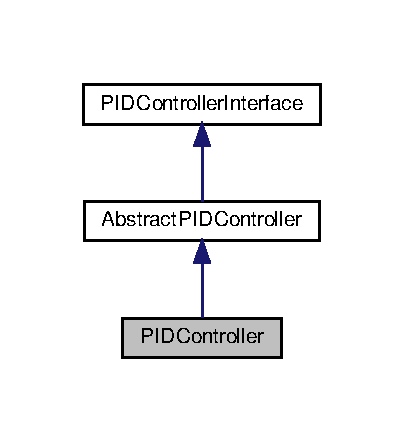
\includegraphics[width=194pt]{classPIDController__coll__graph}
\end{center}
\end{figure}
\subsection*{Public Member Functions}
\begin{DoxyCompactItemize}
\item 
\hyperlink{classPIDController_aba84b9949f9e74bf038cc0a5a7ad7c67}{P\+I\+D\+Controller} (double kP, double kI, double kD, double max\+\_\+value, double min\+\_\+value, double dt)
\begin{DoxyCompactList}\small\item\em Construct a new \hyperlink{classPIDController}{P\+I\+D\+Controller} object. \end{DoxyCompactList}\item 
\mbox{\Hypertarget{classPIDController_a690e7ad4796e5c5143aa4b90f2f6677b}\label{classPIDController_a690e7ad4796e5c5143aa4b90f2f6677b}} 
\hyperlink{classPIDController_a690e7ad4796e5c5143aa4b90f2f6677b}{$\sim$\+P\+I\+D\+Controller} ()
\begin{DoxyCompactList}\small\item\em Destroy the \hyperlink{classPIDController}{P\+I\+D\+Controller} object. \end{DoxyCompactList}\item 
double \hyperlink{classPIDController_a0b57631654b460a4668f01b7cc0c8ecb}{compute} (double setpoint\+\_\+value, double measured\+\_\+value) override
\item 
double \hyperlink{classPIDController_a338490568fd2de02c4e1eea130a816c1}{get\+\_\+dt} () const override
\begin{DoxyCompactList}\small\item\em Get sampling time -\/ dt. \end{DoxyCompactList}\item 
void \hyperlink{classPIDController_a04c753e2ff22f62017f82e0e4143493b}{set\+\_\+dt} (double dt) override
\begin{DoxyCompactList}\small\item\em Set sampling time -\/ dt. \end{DoxyCompactList}\item 
double \hyperlink{classPIDController_a0f366ed8608947fa17454682773a48ee}{get\+\_\+kD} () const override
\begin{DoxyCompactList}\small\item\em Get value of differential gain kD. \end{DoxyCompactList}\item 
void \hyperlink{classPIDController_a88adb39de00d22b72a8a33716fc1c117}{set\+\_\+kD} (double kD) override
\begin{DoxyCompactList}\small\item\em Set value of differential gain kD. \end{DoxyCompactList}\item 
double \hyperlink{classPIDController_af79b88e9f6c99667fb1474219f00f6f3}{get\+\_\+kI} () const override
\begin{DoxyCompactList}\small\item\em Get value of integral gain kI. \end{DoxyCompactList}\item 
void \hyperlink{classPIDController_a5724db51f8d64e8adf5c6f466dc66d8c}{set\+\_\+kI} (double kI) override
\begin{DoxyCompactList}\small\item\em Set value of integral gain kI. \end{DoxyCompactList}\item 
double \hyperlink{classPIDController_ac838d1c775ff75c7845602b189e5f214}{get\+\_\+kP} () const
\begin{DoxyCompactList}\small\item\em Get value of proportional gain kP. \end{DoxyCompactList}\item 
void \hyperlink{classPIDController_a7b97f2fa293347e9e9391d5ca3b80e8b}{set\+\_\+kP} (double kP)
\begin{DoxyCompactList}\small\item\em Set value of proportional gain kP. \end{DoxyCompactList}\item 
double \hyperlink{classPIDController_ad4420e831743f6b66303f6a24bf7fbdc}{get\+\_\+max\+\_\+value} () const
\begin{DoxyCompactList}\small\item\em Get the max value for the parameter. \end{DoxyCompactList}\item 
void \hyperlink{classPIDController_a942161494e6b3bc4996e688f390a59bf}{set\+\_\+max\+\_\+value} (double max\+Value)
\begin{DoxyCompactList}\small\item\em Set the max value for the parameter. \end{DoxyCompactList}\item 
double \hyperlink{classPIDController_ab29545c6bcce3ef804bdbf0f2441cb4e}{get\+\_\+min\+\_\+value} () const
\begin{DoxyCompactList}\small\item\em Get the min value for the parameter. \end{DoxyCompactList}\item 
void \hyperlink{classPIDController_a101d69b58ee371c45b1046dcd2bd58e7}{set\+\_\+min\+\_\+value} (double min\+Value)
\begin{DoxyCompactList}\small\item\em Set the min value for the parameter. \end{DoxyCompactList}\item 
double \hyperlink{classPIDController_a7617f92c27f92fa53e8c690a721e9965}{get\+\_\+prev\+\_\+error} () const
\begin{DoxyCompactList}\small\item\em Get the prev\+\_\+error. \end{DoxyCompactList}\item 
double \hyperlink{classPIDController_a9f5ea16a313044807fbd23135646c88e}{get\+\_\+integral\+\_\+sum} () const
\begin{DoxyCompactList}\small\item\em Get the integral\+\_\+sum over time. \end{DoxyCompactList}\end{DoxyCompactItemize}


\subsection{Detailed Description}
Concrete implementation of the \hyperlink{classPIDController}{P\+I\+D\+Controller} abstract class and interface. 

\subsection{Constructor \& Destructor Documentation}
\mbox{\Hypertarget{classPIDController_aba84b9949f9e74bf038cc0a5a7ad7c67}\label{classPIDController_aba84b9949f9e74bf038cc0a5a7ad7c67}} 
\index{P\+I\+D\+Controller@{P\+I\+D\+Controller}!P\+I\+D\+Controller@{P\+I\+D\+Controller}}
\index{P\+I\+D\+Controller@{P\+I\+D\+Controller}!P\+I\+D\+Controller@{P\+I\+D\+Controller}}
\subsubsection{\texorpdfstring{P\+I\+D\+Controller()}{PIDController()}}
{\footnotesize\ttfamily P\+I\+D\+Controller\+::\+P\+I\+D\+Controller (\begin{DoxyParamCaption}\item[{double}]{kP,  }\item[{double}]{kI,  }\item[{double}]{kD,  }\item[{double}]{max\+\_\+value,  }\item[{double}]{min\+\_\+value,  }\item[{double}]{dt }\end{DoxyParamCaption})}



Construct a new \hyperlink{classPIDController}{P\+I\+D\+Controller} object. 


\begin{DoxyParams}{Parameters}
{\em kP} & proportional gain \\
\hline
{\em kI} & integral gain \\
\hline
{\em kD} & differential gain \\
\hline
{\em max\+\_\+value} & maximum value that the parameter (ex\+: velocity) can have \\
\hline
{\em min\+\_\+value} & minimum value that the parameter (ex\+: velocity) can have \\
\hline
{\em dt} & sampling time\\
\hline
\end{DoxyParams}
Copyright 2021 Anubhav Paras, Charu Sharma, Arunava Basu \& Shon Cortes  Part 1\+: Design\+:
\begin{DoxyItemize}
\item Driver\+: Anubhav Paras
\item Navigator\+: Charu Sharma
\end{DoxyItemize}

Part 2\+: Implementation\+:
\begin{DoxyItemize}
\item Driver\+: Shon Cortes
\item Navigator\+: Arunava Basu 
\end{DoxyItemize}

\subsection{Member Function Documentation}
\mbox{\Hypertarget{classPIDController_a0b57631654b460a4668f01b7cc0c8ecb}\label{classPIDController_a0b57631654b460a4668f01b7cc0c8ecb}} 
\index{P\+I\+D\+Controller@{P\+I\+D\+Controller}!compute@{compute}}
\index{compute@{compute}!P\+I\+D\+Controller@{P\+I\+D\+Controller}}
\subsubsection{\texorpdfstring{compute()}{compute()}}
{\footnotesize\ttfamily double P\+I\+D\+Controller\+::compute (\begin{DoxyParamCaption}\item[{double}]{setpoint\+\_\+value,  }\item[{double}]{measured\+\_\+value }\end{DoxyParamCaption})\hspace{0.3cm}{\ttfamily [override]}, {\ttfamily [virtual]}}


\begin{DoxyParams}{Parameters}
{\em setpoint\+\_\+value} & target value of the parameter \\
\hline
{\em measured\+\_\+value} & current measured estimate of the parameter \\
\hline
\end{DoxyParams}
\begin{DoxyReturn}{Returns}
double 
\end{DoxyReturn}


Implements \hyperlink{classPIDControllerInterface_a6b5340968cb9d235cf3b52bd61c973e1}{P\+I\+D\+Controller\+Interface}.

\mbox{\Hypertarget{classPIDController_a338490568fd2de02c4e1eea130a816c1}\label{classPIDController_a338490568fd2de02c4e1eea130a816c1}} 
\index{P\+I\+D\+Controller@{P\+I\+D\+Controller}!get\+\_\+dt@{get\+\_\+dt}}
\index{get\+\_\+dt@{get\+\_\+dt}!P\+I\+D\+Controller@{P\+I\+D\+Controller}}
\subsubsection{\texorpdfstring{get\+\_\+dt()}{get\_dt()}}
{\footnotesize\ttfamily double P\+I\+D\+Controller\+::get\+\_\+dt (\begin{DoxyParamCaption}{ }\end{DoxyParamCaption}) const\hspace{0.3cm}{\ttfamily [override]}, {\ttfamily [virtual]}}



Get sampling time -\/ dt. 

\begin{DoxyReturn}{Returns}
double 
\end{DoxyReturn}


Implements \hyperlink{classAbstractPIDController}{Abstract\+P\+I\+D\+Controller}.

\mbox{\Hypertarget{classPIDController_a9f5ea16a313044807fbd23135646c88e}\label{classPIDController_a9f5ea16a313044807fbd23135646c88e}} 
\index{P\+I\+D\+Controller@{P\+I\+D\+Controller}!get\+\_\+integral\+\_\+sum@{get\+\_\+integral\+\_\+sum}}
\index{get\+\_\+integral\+\_\+sum@{get\+\_\+integral\+\_\+sum}!P\+I\+D\+Controller@{P\+I\+D\+Controller}}
\subsubsection{\texorpdfstring{get\+\_\+integral\+\_\+sum()}{get\_integral\_sum()}}
{\footnotesize\ttfamily double P\+I\+D\+Controller\+::get\+\_\+integral\+\_\+sum (\begin{DoxyParamCaption}{ }\end{DoxyParamCaption}) const\hspace{0.3cm}{\ttfamily [virtual]}}



Get the integral\+\_\+sum over time. 

\begin{DoxyReturn}{Returns}
double 
\end{DoxyReturn}


Implements \hyperlink{classAbstractPIDController}{Abstract\+P\+I\+D\+Controller}.

\mbox{\Hypertarget{classPIDController_a0f366ed8608947fa17454682773a48ee}\label{classPIDController_a0f366ed8608947fa17454682773a48ee}} 
\index{P\+I\+D\+Controller@{P\+I\+D\+Controller}!get\+\_\+kD@{get\+\_\+kD}}
\index{get\+\_\+kD@{get\+\_\+kD}!P\+I\+D\+Controller@{P\+I\+D\+Controller}}
\subsubsection{\texorpdfstring{get\+\_\+k\+D()}{get\_kD()}}
{\footnotesize\ttfamily double P\+I\+D\+Controller\+::get\+\_\+kD (\begin{DoxyParamCaption}{ }\end{DoxyParamCaption}) const\hspace{0.3cm}{\ttfamily [override]}, {\ttfamily [virtual]}}



Get value of differential gain kD. 

\begin{DoxyReturn}{Returns}
double 
\end{DoxyReturn}


Implements \hyperlink{classAbstractPIDController}{Abstract\+P\+I\+D\+Controller}.

\mbox{\Hypertarget{classPIDController_af79b88e9f6c99667fb1474219f00f6f3}\label{classPIDController_af79b88e9f6c99667fb1474219f00f6f3}} 
\index{P\+I\+D\+Controller@{P\+I\+D\+Controller}!get\+\_\+kI@{get\+\_\+kI}}
\index{get\+\_\+kI@{get\+\_\+kI}!P\+I\+D\+Controller@{P\+I\+D\+Controller}}
\subsubsection{\texorpdfstring{get\+\_\+k\+I()}{get\_kI()}}
{\footnotesize\ttfamily double P\+I\+D\+Controller\+::get\+\_\+kI (\begin{DoxyParamCaption}{ }\end{DoxyParamCaption}) const\hspace{0.3cm}{\ttfamily [override]}, {\ttfamily [virtual]}}



Get value of integral gain kI. 

\begin{DoxyReturn}{Returns}
double 
\end{DoxyReturn}


Implements \hyperlink{classAbstractPIDController}{Abstract\+P\+I\+D\+Controller}.

\mbox{\Hypertarget{classPIDController_ac838d1c775ff75c7845602b189e5f214}\label{classPIDController_ac838d1c775ff75c7845602b189e5f214}} 
\index{P\+I\+D\+Controller@{P\+I\+D\+Controller}!get\+\_\+kP@{get\+\_\+kP}}
\index{get\+\_\+kP@{get\+\_\+kP}!P\+I\+D\+Controller@{P\+I\+D\+Controller}}
\subsubsection{\texorpdfstring{get\+\_\+k\+P()}{get\_kP()}}
{\footnotesize\ttfamily double P\+I\+D\+Controller\+::get\+\_\+kP (\begin{DoxyParamCaption}{ }\end{DoxyParamCaption}) const\hspace{0.3cm}{\ttfamily [virtual]}}



Get value of proportional gain kP. 

\begin{DoxyReturn}{Returns}
double 
\end{DoxyReturn}


Implements \hyperlink{classAbstractPIDController}{Abstract\+P\+I\+D\+Controller}.

\mbox{\Hypertarget{classPIDController_ad4420e831743f6b66303f6a24bf7fbdc}\label{classPIDController_ad4420e831743f6b66303f6a24bf7fbdc}} 
\index{P\+I\+D\+Controller@{P\+I\+D\+Controller}!get\+\_\+max\+\_\+value@{get\+\_\+max\+\_\+value}}
\index{get\+\_\+max\+\_\+value@{get\+\_\+max\+\_\+value}!P\+I\+D\+Controller@{P\+I\+D\+Controller}}
\subsubsection{\texorpdfstring{get\+\_\+max\+\_\+value()}{get\_max\_value()}}
{\footnotesize\ttfamily double P\+I\+D\+Controller\+::get\+\_\+max\+\_\+value (\begin{DoxyParamCaption}{ }\end{DoxyParamCaption}) const\hspace{0.3cm}{\ttfamily [virtual]}}



Get the max value for the parameter. 

\begin{DoxyReturn}{Returns}
double 
\end{DoxyReturn}


Implements \hyperlink{classAbstractPIDController}{Abstract\+P\+I\+D\+Controller}.

\mbox{\Hypertarget{classPIDController_ab29545c6bcce3ef804bdbf0f2441cb4e}\label{classPIDController_ab29545c6bcce3ef804bdbf0f2441cb4e}} 
\index{P\+I\+D\+Controller@{P\+I\+D\+Controller}!get\+\_\+min\+\_\+value@{get\+\_\+min\+\_\+value}}
\index{get\+\_\+min\+\_\+value@{get\+\_\+min\+\_\+value}!P\+I\+D\+Controller@{P\+I\+D\+Controller}}
\subsubsection{\texorpdfstring{get\+\_\+min\+\_\+value()}{get\_min\_value()}}
{\footnotesize\ttfamily double P\+I\+D\+Controller\+::get\+\_\+min\+\_\+value (\begin{DoxyParamCaption}{ }\end{DoxyParamCaption}) const\hspace{0.3cm}{\ttfamily [virtual]}}



Get the min value for the parameter. 

\begin{DoxyReturn}{Returns}
double 
\end{DoxyReturn}


Implements \hyperlink{classAbstractPIDController}{Abstract\+P\+I\+D\+Controller}.

\mbox{\Hypertarget{classPIDController_a7617f92c27f92fa53e8c690a721e9965}\label{classPIDController_a7617f92c27f92fa53e8c690a721e9965}} 
\index{P\+I\+D\+Controller@{P\+I\+D\+Controller}!get\+\_\+prev\+\_\+error@{get\+\_\+prev\+\_\+error}}
\index{get\+\_\+prev\+\_\+error@{get\+\_\+prev\+\_\+error}!P\+I\+D\+Controller@{P\+I\+D\+Controller}}
\subsubsection{\texorpdfstring{get\+\_\+prev\+\_\+error()}{get\_prev\_error()}}
{\footnotesize\ttfamily double P\+I\+D\+Controller\+::get\+\_\+prev\+\_\+error (\begin{DoxyParamCaption}{ }\end{DoxyParamCaption}) const\hspace{0.3cm}{\ttfamily [virtual]}}



Get the prev\+\_\+error. 

\begin{DoxyReturn}{Returns}
double 
\end{DoxyReturn}


Implements \hyperlink{classAbstractPIDController}{Abstract\+P\+I\+D\+Controller}.

\mbox{\Hypertarget{classPIDController_a04c753e2ff22f62017f82e0e4143493b}\label{classPIDController_a04c753e2ff22f62017f82e0e4143493b}} 
\index{P\+I\+D\+Controller@{P\+I\+D\+Controller}!set\+\_\+dt@{set\+\_\+dt}}
\index{set\+\_\+dt@{set\+\_\+dt}!P\+I\+D\+Controller@{P\+I\+D\+Controller}}
\subsubsection{\texorpdfstring{set\+\_\+dt()}{set\_dt()}}
{\footnotesize\ttfamily void P\+I\+D\+Controller\+::set\+\_\+dt (\begin{DoxyParamCaption}\item[{double}]{dt }\end{DoxyParamCaption})\hspace{0.3cm}{\ttfamily [override]}, {\ttfamily [virtual]}}



Set sampling time -\/ dt. 


\begin{DoxyParams}{Parameters}
{\em dt} & \\
\hline
\end{DoxyParams}


Implements \hyperlink{classAbstractPIDController}{Abstract\+P\+I\+D\+Controller}.

\mbox{\Hypertarget{classPIDController_a88adb39de00d22b72a8a33716fc1c117}\label{classPIDController_a88adb39de00d22b72a8a33716fc1c117}} 
\index{P\+I\+D\+Controller@{P\+I\+D\+Controller}!set\+\_\+kD@{set\+\_\+kD}}
\index{set\+\_\+kD@{set\+\_\+kD}!P\+I\+D\+Controller@{P\+I\+D\+Controller}}
\subsubsection{\texorpdfstring{set\+\_\+k\+D()}{set\_kD()}}
{\footnotesize\ttfamily void P\+I\+D\+Controller\+::set\+\_\+kD (\begin{DoxyParamCaption}\item[{double}]{kD }\end{DoxyParamCaption})\hspace{0.3cm}{\ttfamily [override]}, {\ttfamily [virtual]}}



Set value of differential gain kD. 


\begin{DoxyParams}{Parameters}
{\em kD} & \\
\hline
\end{DoxyParams}


Implements \hyperlink{classAbstractPIDController}{Abstract\+P\+I\+D\+Controller}.

\mbox{\Hypertarget{classPIDController_a5724db51f8d64e8adf5c6f466dc66d8c}\label{classPIDController_a5724db51f8d64e8adf5c6f466dc66d8c}} 
\index{P\+I\+D\+Controller@{P\+I\+D\+Controller}!set\+\_\+kI@{set\+\_\+kI}}
\index{set\+\_\+kI@{set\+\_\+kI}!P\+I\+D\+Controller@{P\+I\+D\+Controller}}
\subsubsection{\texorpdfstring{set\+\_\+k\+I()}{set\_kI()}}
{\footnotesize\ttfamily void P\+I\+D\+Controller\+::set\+\_\+kI (\begin{DoxyParamCaption}\item[{double}]{kI }\end{DoxyParamCaption})\hspace{0.3cm}{\ttfamily [override]}, {\ttfamily [virtual]}}



Set value of integral gain kI. 


\begin{DoxyParams}{Parameters}
{\em kI} & \\
\hline
\end{DoxyParams}


Implements \hyperlink{classAbstractPIDController}{Abstract\+P\+I\+D\+Controller}.

\mbox{\Hypertarget{classPIDController_a7b97f2fa293347e9e9391d5ca3b80e8b}\label{classPIDController_a7b97f2fa293347e9e9391d5ca3b80e8b}} 
\index{P\+I\+D\+Controller@{P\+I\+D\+Controller}!set\+\_\+kP@{set\+\_\+kP}}
\index{set\+\_\+kP@{set\+\_\+kP}!P\+I\+D\+Controller@{P\+I\+D\+Controller}}
\subsubsection{\texorpdfstring{set\+\_\+k\+P()}{set\_kP()}}
{\footnotesize\ttfamily void P\+I\+D\+Controller\+::set\+\_\+kP (\begin{DoxyParamCaption}\item[{double}]{kP }\end{DoxyParamCaption})\hspace{0.3cm}{\ttfamily [virtual]}}



Set value of proportional gain kP. 


\begin{DoxyParams}{Parameters}
{\em kP} & \\
\hline
\end{DoxyParams}


Implements \hyperlink{classAbstractPIDController}{Abstract\+P\+I\+D\+Controller}.

\mbox{\Hypertarget{classPIDController_a942161494e6b3bc4996e688f390a59bf}\label{classPIDController_a942161494e6b3bc4996e688f390a59bf}} 
\index{P\+I\+D\+Controller@{P\+I\+D\+Controller}!set\+\_\+max\+\_\+value@{set\+\_\+max\+\_\+value}}
\index{set\+\_\+max\+\_\+value@{set\+\_\+max\+\_\+value}!P\+I\+D\+Controller@{P\+I\+D\+Controller}}
\subsubsection{\texorpdfstring{set\+\_\+max\+\_\+value()}{set\_max\_value()}}
{\footnotesize\ttfamily void P\+I\+D\+Controller\+::set\+\_\+max\+\_\+value (\begin{DoxyParamCaption}\item[{double}]{max\+Value }\end{DoxyParamCaption})\hspace{0.3cm}{\ttfamily [virtual]}}



Set the max value for the parameter. 


\begin{DoxyParams}{Parameters}
{\em max\+Value} & \\
\hline
\end{DoxyParams}


Implements \hyperlink{classAbstractPIDController}{Abstract\+P\+I\+D\+Controller}.

\mbox{\Hypertarget{classPIDController_a101d69b58ee371c45b1046dcd2bd58e7}\label{classPIDController_a101d69b58ee371c45b1046dcd2bd58e7}} 
\index{P\+I\+D\+Controller@{P\+I\+D\+Controller}!set\+\_\+min\+\_\+value@{set\+\_\+min\+\_\+value}}
\index{set\+\_\+min\+\_\+value@{set\+\_\+min\+\_\+value}!P\+I\+D\+Controller@{P\+I\+D\+Controller}}
\subsubsection{\texorpdfstring{set\+\_\+min\+\_\+value()}{set\_min\_value()}}
{\footnotesize\ttfamily void P\+I\+D\+Controller\+::set\+\_\+min\+\_\+value (\begin{DoxyParamCaption}\item[{double}]{min\+Value }\end{DoxyParamCaption})\hspace{0.3cm}{\ttfamily [virtual]}}



Set the min value for the parameter. 


\begin{DoxyParams}{Parameters}
{\em min\+Value} & \\
\hline
\end{DoxyParams}


Implements \hyperlink{classAbstractPIDController}{Abstract\+P\+I\+D\+Controller}.



The documentation for this class was generated from the following files\+:\begin{DoxyCompactItemize}
\item 
include/pid.\+hpp\item 
src/pid.\+cpp\end{DoxyCompactItemize}

\hypertarget{classPIDControllerInterface}{}\section{P\+I\+D\+Controller\+Interface Class Reference}
\label{classPIDControllerInterface}\index{P\+I\+D\+Controller\+Interface@{P\+I\+D\+Controller\+Interface}}


\hyperlink{classPIDController}{P\+I\+D\+Controller} interface will have the \hyperlink{classPIDControllerInterface_a6b5340968cb9d235cf3b52bd61c973e1}{compute()} method. This can be implemented by any concrete class.  




{\ttfamily \#include $<$pid.\+hpp$>$}



Inheritance diagram for P\+I\+D\+Controller\+Interface\+:\nopagebreak
\begin{figure}[H]
\begin{center}
\leavevmode
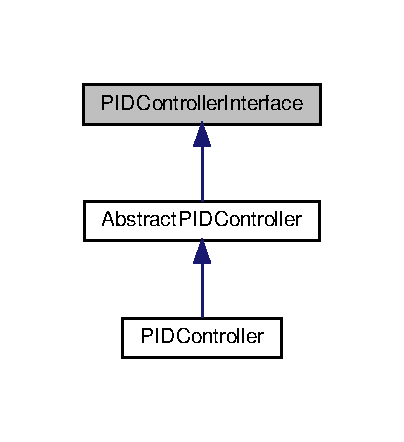
\includegraphics[width=194pt]{classPIDControllerInterface__inherit__graph}
\end{center}
\end{figure}
\subsection*{Public Member Functions}
\begin{DoxyCompactItemize}
\item 
virtual double \hyperlink{classPIDControllerInterface_a6b5340968cb9d235cf3b52bd61c973e1}{compute} (double setpoint\+\_\+value, double measured\+\_\+value)=0
\begin{DoxyCompactList}\small\item\em To find the controller output value based on the target setpoint and measured values. \end{DoxyCompactList}\item 
\mbox{\Hypertarget{classPIDControllerInterface_a96ae6d60601a238ddf999cee5fe705a0}\label{classPIDControllerInterface_a96ae6d60601a238ddf999cee5fe705a0}} 
virtual \hyperlink{classPIDControllerInterface_a96ae6d60601a238ddf999cee5fe705a0}{$\sim$\+P\+I\+D\+Controller\+Interface} ()
\begin{DoxyCompactList}\small\item\em Destroy the \hyperlink{classPIDControllerInterface}{P\+I\+D\+Controller\+Interface} object. \end{DoxyCompactList}\end{DoxyCompactItemize}


\subsection{Detailed Description}
\hyperlink{classPIDController}{P\+I\+D\+Controller} interface will have the \hyperlink{classPIDControllerInterface_a6b5340968cb9d235cf3b52bd61c973e1}{compute()} method. This can be implemented by any concrete class. 

Copyright 2021 Anubhav Paras, Charu Sharma, Arunava Basu \& Shon Cortes  Part 1\+: Design\+:
\begin{DoxyItemize}
\item Driver\+: Anubhav Paras
\item Navigator\+: Charu Sharma
\end{DoxyItemize}

Part 2\+: Implementation\+:
\begin{DoxyItemize}
\item Driver\+: Shon Cortes
\item Navigator\+: Arunava Basu 
\end{DoxyItemize}

\subsection{Member Function Documentation}
\mbox{\Hypertarget{classPIDControllerInterface_a6b5340968cb9d235cf3b52bd61c973e1}\label{classPIDControllerInterface_a6b5340968cb9d235cf3b52bd61c973e1}} 
\index{P\+I\+D\+Controller\+Interface@{P\+I\+D\+Controller\+Interface}!compute@{compute}}
\index{compute@{compute}!P\+I\+D\+Controller\+Interface@{P\+I\+D\+Controller\+Interface}}
\subsubsection{\texorpdfstring{compute()}{compute()}}
{\footnotesize\ttfamily virtual double P\+I\+D\+Controller\+Interface\+::compute (\begin{DoxyParamCaption}\item[{double}]{setpoint\+\_\+value,  }\item[{double}]{measured\+\_\+value }\end{DoxyParamCaption})\hspace{0.3cm}{\ttfamily [pure virtual]}}



To find the controller output value based on the target setpoint and measured values. 


\begin{DoxyParams}{Parameters}
{\em setpoint\+\_\+value} & target value of the parameter \\
\hline
{\em measured\+\_\+value} & current measured estimate of the parameter \\
\hline
\end{DoxyParams}
\begin{DoxyReturn}{Returns}
double 
\end{DoxyReturn}


Implemented in \hyperlink{classPIDController_a0b57631654b460a4668f01b7cc0c8ecb}{P\+I\+D\+Controller}.



The documentation for this class was generated from the following file\+:\begin{DoxyCompactItemize}
\item 
include/pid.\+hpp\end{DoxyCompactItemize}

%--- End generated contents ---

% Index
\backmatter
\newpage
\phantomsection
\clearemptydoublepage
\addcontentsline{toc}{chapter}{Index}
\printindex

\end{document}
